\documentclass[11pt]{article}
% \usepackage{times}
\usepackage{palatino}
\usepackage{colortbl}

\usepackage{tikz}
\usetikzlibrary{shapes.geometric, arrows}
\tikzstyle{startstop} = [rectangle, rounded corners, minimum width=3cm, minimum height=1cm,text centered, draw=black, fill=red!30]
\tikzstyle{io} = [trapezium, trapezium left angle=70, trapezium right angle=110, minimum width=3cm, minimum height=1cm, text centered, draw=black, fill=blue!30]
\tikzstyle{process} = [rectangle, minimum width=3cm, minimum height=1cm, text centered, draw=black, fill=orange!30]
\tikzstyle{decision} = [diamond, minimum width=3cm, minimum height=1cm, text centered, draw=black, fill=green!30]
\tikzstyle{arrow} = [thick,->,>=stealth]

\renewcommand{\baselinestretch}{1.2} 
\setlength{\topmargin}{-1.0in}
\setlength{\textwidth}{6.5in}
\setlength{\oddsidemargin}{0.0in}
\setlength{\textheight}{10.1in}

\newlength{\pagewidth}
\setlength{\pagewidth}{6.5in}
\pagestyle{empty}

\def\pp{\par\noindent}

\special{papersize=8.5in,11in}


\begin{document}
\noindent 
Tony Li \\
CSE150 \\
HW01b \\\\
%=========================================Problem 4=====================================================
	\textbf{\underline{Problem 4:}}


	Boolean algebra operations can be expressed as arithmetic operations mod 2. Let 1 represent 

	true, and 0 false.

	( a ) Show that A $\wedge$ B = ( A $\bullet$ B mod 2 ).\\

	\begin{minipage}{0.5\textwidth}
		\begin{tabular}{||c c c||} 
 		\hline
 		A & B & A $\wedge$ B\\ [0.5ex] 
 		\hline\hline
 		T & T & T\\ 
 		\hline
 		T & F & F\\
 		\hline
 		F & T & F\\
 		\hline
 		F & F & F\\
 		\hline
		\end{tabular}
	\end{minipage}
	\begin{minipage}{0.5\textwidth}
		\begin{tabular}{||c c c||} 
 		\hline
 		A & B & A $\bullet$ B mod 2\\ [0.5ex] 
 		\hline\hline
 		1 & 1 & 1\\ 
 		\hline
 		1 & 0 & 0\\
 		\hline
 		0 & 1 & 0\\
 		\hline
 		0 & 0 & 0\\
 		\hline
		\end{tabular}
	\end{minipage}\\\\

	( b ) What is $\sim$A?\\

	\begin{tabular}{||c c c c||} 
 		\hline
 		A & $\sim$A & A+1 & A+1 mod 2\\ [0.5ex] 
 		\hline\hline
 		1 & 0 & 2 & 0\\ 
 		\hline
 		1 & 0 & 2 & 0\\
 		\hline
 		0 & 1 & 1 & 1\\
 		\hline
 		0 & 1 & 1 & 1\\
 		\hline
		\end{tabular}\\\\

	( c ) What is A $\vee$ B? (Use De Morgan's laws.)\\
	\begin{enumerate}
		\item A $\vee$ B
		\item $\sim$ ( $\sim$A $\wedge$ $\sim$B) \textit{[by De Morgan's Laws]}
		\item $\sim$( $\sim$A $\bullet\sim$B )$\bmod$2  \textit{[by Problem 4a]}
		\item ( ( A + 1 ) $\bmod$2 $\bullet$ ( B + 1 )$\bmod$2 + 1 )$\bmod$2 \textit{[by Problem 4b]}
	\end{enumerate}
\   \\\\\\\\\\\\\\\\\\\\\\\\
%=========================================Problem 5a=====================================================
	\noindent\textbf{\underline{Problem 5:}}

	Over lunch at the faculty club, $n$ professors are expressing their concerns over their salaries. 

	Each professor wants to know how his/her salary compares to the average salary of the group,

	but no professor wants to divulge any information about his/her salary to the other $n - 1$.\\

	( a ) Devise a scheme that allows the professors to compute the avergae of their salaries, while
	
	preserving their privacy.\\

	You may assume that all the professors will adhere to the rules of the protocol, although they 

	will try to extract as much information form the profoud as possible. You may also assume 

	that it is public knowledge that the professors' salaries together don't exceed \$1 trillion.
	\\\\\\
	The first professor chooses an arbitrary number from 0 to a very very large number $L$. 
	Lets call that number $R$ and the first professor's salary $S_1$.  We will sum $S_1$ and $R$ 
	and then pass it on to the next professor who will add his/her salary to it. \textbf{However, this 
	reveals information since the expected value of the sum is $L/2$ .}
	\\\\
	Why?
	\\\\
	Any number from $0\rightarrow L-1$ is considered a random number, including the first professor's salary. The sum of two random numbers is not truly random because the set of sums is normally distributed. 
	\\\\
	Solution.
	\\\\
	We can mod the sum by $L$ so that the sums that are greater than $L-1$ will be wrapped around. As a result, the set of the modded sum is uniformly distributed.
	\\\\
	We then pass the modded sum, $X_1$, to the 2nd professor and he will add his salary to the modded sum; $X_1+S_2=X_2$. He passes it to the 3rd professor and professor 3's salary will be added to the sum;$X_2+S_3=X_3$. We repeat this until the sum gets to the $n^{th}$ professor who will pass the final sum, $X_n$, to the first professor. He subtracts the random number from $X_n$ to get the sum of the salaries and divides it by $N$ to get the average salary.
	\\\\\\\\\\\\\\\\\\\\\\
%=========================================Problem 5b=====================================================
	( b ) Now extend the protocol to be robust even when groups of professors collude. Specifically, if $i$ professors collude, naturally, naturally they can learn the average salary of the remaining $n - i$. Your protocol should reveal no additional information.
	\\\\\\
	We can build upon solution (5a) by letting each professor choose a random number, instead of only the first professor. The first professor passes his modded sum, $X_1$, like usual to the second. However, this time the second professor will add his salary and his random number to $X_1$ and mod the new sum by $L$. This will repeat until $\Sigma$ Salaries + $\Sigma$ Random\#s reaches the first professor.
	\\\\
	\textbf{Example with 4 professors}
	\\\\
	\begin{tikzpicture}[node distance=2cm]

	\node (p1) [startstop] {Professor 1};
	\node (p2) [startstop, right of=p1, xshift=6cm] {Professor 2};
	\node (p3) [startstop, below of=p2, yshift=-1cm]{Professor 3};
	\node (p4) [startstop, left of=p3, xshift=-6cm]{Professor 4};

	\draw [arrow] (p1) -- node[anchor = south]{$S_1 +_{L} R_1 = X_1$}(p2);
	\draw [arrow] (p2) -- node[anchor = west]{$X_1 +_{L} S_2 +_{L} R_2 = X_2$}(p3);
	\draw [arrow] (p3) -- node[anchor = north]{$X_2 +_{L} S_3 +_{L} R_3 = X_3$}(p4);
	\draw [arrow] (p4) -- node[anchor = east]{$X_3 +_{L} S_4 +_{L} R_4 = X_4$}(p1);
	\end{tikzpicture}
	\\\\
	Next, each professor will split their random number into a sum of $n-1$ terms. Then they will assign each term to another professor. Each professor will have a pool of terms, each from a different professor. They will sum their terms. The first professor will subtract his sum from the number he received last, $\Sigma$ Salaries + $\Sigma$ Random\#s and mod the difference by $L$ to take care of negative differences. He then passes the difference to the 2nd Professor, and he does the same thing. This repeats until it gets to the first, who gets the sum of the salaries when the $n^{th}$ professor subtracts his sum of terms and divides the sum by $n$ to get the average. Let $D_n$ represent the sum of the terms each professor gets and $Y_n$ represent the difference between the last number and $D_n$.
	\\
	$\Sigma R = R_1 + R_2 + R_3 + R_4 = D_1 + D_2 + D_3 + D_4$\\\\
	\begin{minipage}{0.5\textwidth}
	Professor 1: $R_1 = r_{11} + r_{12} + r_{13}$ \\
	Professor 2: $R_2 = r_{21} + r_{22} + r_{23}$ \\
	Professor 3: $R_3 = r_{31} + r_{32} + r_{33}$ \\
	Professor 4: $R_4 = r_{41} + r_{42} + r_{43}$ 

	\end{minipage}
	\begin{minipage}{0.5\textwidth}
	
	Professor 1: $D_1= r_{21} + r_{31} + r_{41}$ \\
	Professor 2: $D_2 = r_{11} + r_{32} + r_{42}$ \\
	Professor 3: $D_3 = r_{12} + r_{22} + r_{43}$ \\
	Professor 4: $D_4 = r_{13} + r_{21} + r_{33}$ 
	\end{minipage}

	\begin{tikzpicture}[node distance=2cm]

	\node (p1) [startstop] {Professor 1};
	\node (p2) [startstop, right of=p1, xshift=6cm] {Professor 2};
	\node (p3) [startstop, below of=p2, yshift=-1cm]{Professor 3};
	\node (p4) [startstop, left of=p3, xshift=-6cm]{Professor 4};

	\draw [arrow] (p1) -- node[anchor = south]{$X_4 -_{L} D_1 = Y_1$}(p2);
	\draw [arrow] (p2) -- node[anchor = west]{$Y_1 -_{L} D_2 = Y_2$}(p3);
	\draw [arrow] (p3) -- node[anchor = north]{$Y_2 -_{L} D_3 = Y_3$}(p4);
	\draw [arrow] (p4) -- node[anchor = east]{$Y_3 -_{L} D_4 = Y_4 = \Sigma S$}(p1);
	\end{tikzpicture}
	\\
	***Collaborated with Raymond Wu, Sean Chu, Ivan Lin

	

\end{document}